\documentclass{beamer}
\title{Readers-writers 24/7}
\author{Konrad Kurdej}
\date{18-12-2012}
\usetheme{Hannover}

\AtBeginSection[] { 
  \begin{frame}[plain] 
    \tableofcontents[currentsection] 
  \end{frame}
  \addtocounter{framenumber}{-1} 
}

\definecolor{olive}{rgb}{0.3, 0.4, .1}
\definecolor{fore}{RGB}{249,242,215}
\definecolor{back}{RGB}{51,51,51}
\definecolor{title}{RGB}{255,0,90}
\definecolor{dgreen}{rgb}{0.,0.6,0.}
\definecolor{gold}{rgb}{1.,0.84,0.}
\definecolor{JungleGreen}{cmyk}{0.99,0,0.52,0}
\definecolor{BlueGreen}{cmyk}{0.85,0,0.33,0}
\definecolor{RawSienna}{cmyk}{0,0.72,1,0.45}
\definecolor{Magenta}{cmyk}{0,1,0,0}

\begin{document}
\begin{frame}
\titlepage
\end{frame}
\section*{Outline}
\begin{frame}
\tableofcontents
\end{frame}

\section{Readers-writers}
\begin{frame}
\begin{itemize}
 \item definition (library/data)
 \item fairness / starvation
\end{itemize}
\end{frame}


\section{Fast readers, slow writers}

\begin{frame}
\begin{block}{Why bother?}
\pause
It happens - \textbf{URLAnnotator} aka \textbf{buildaclassifier}.
\end{block}

\pause
\begin{example}[]
\begin{itemize}
 \item reading takes 15 sec, very often (10 per minute)
 \item writing takes 30 min, once an hour
\end{itemize}
\end{example}

\pause
Readers would wait for 30 min ...

\pause
\textcolor{dgreen}{Lets do something about this!}

\end{frame}


\begin{frame}
\frametitle{Lets work with classifier example}

\begin{block}{Classifier operations}
\begin{itemize}
 \item $t$ - train
 \item $c$ - classify\_*
\end{itemize}
\end{block}
Clearly this matches RW schema.

\end{frame}


\begin{frame}
\frametitle{Simple solutions}

\begin{itemize}
 \item create new classifier for each train
 \item do the training
 \item swap newly trained one with \emph{classifying} classifier
\end{itemize}

\pause
\textcolor{RawSienna}{Because we can do better - we won't go into details}

\end{frame}


\begin{frame}
\frametitle{Only two classifiers}

\begin{itemize}
 \item two slots - \textbf{T}rain, \textbf{C}classify
 \item protect \textbf{T} with normal lock/mutex etc.
 \item protect \textbf{C} with RW lock
 \item each classify\_* goes to \textbf{C}
 \item each train goes to \textbf{T}
 \item when we gain lock, we execute command on classifier found in slot
 \item after train, we don't release \textbf{T} lock, we are acquiring \textbf{C} lock and than do swap in slots
\end{itemize}

\pause
\textcolor{JungleGreen}{Let see it in action}

\end{frame}


\begin{frame}
\frametitle{Overall view}
\begin{center}
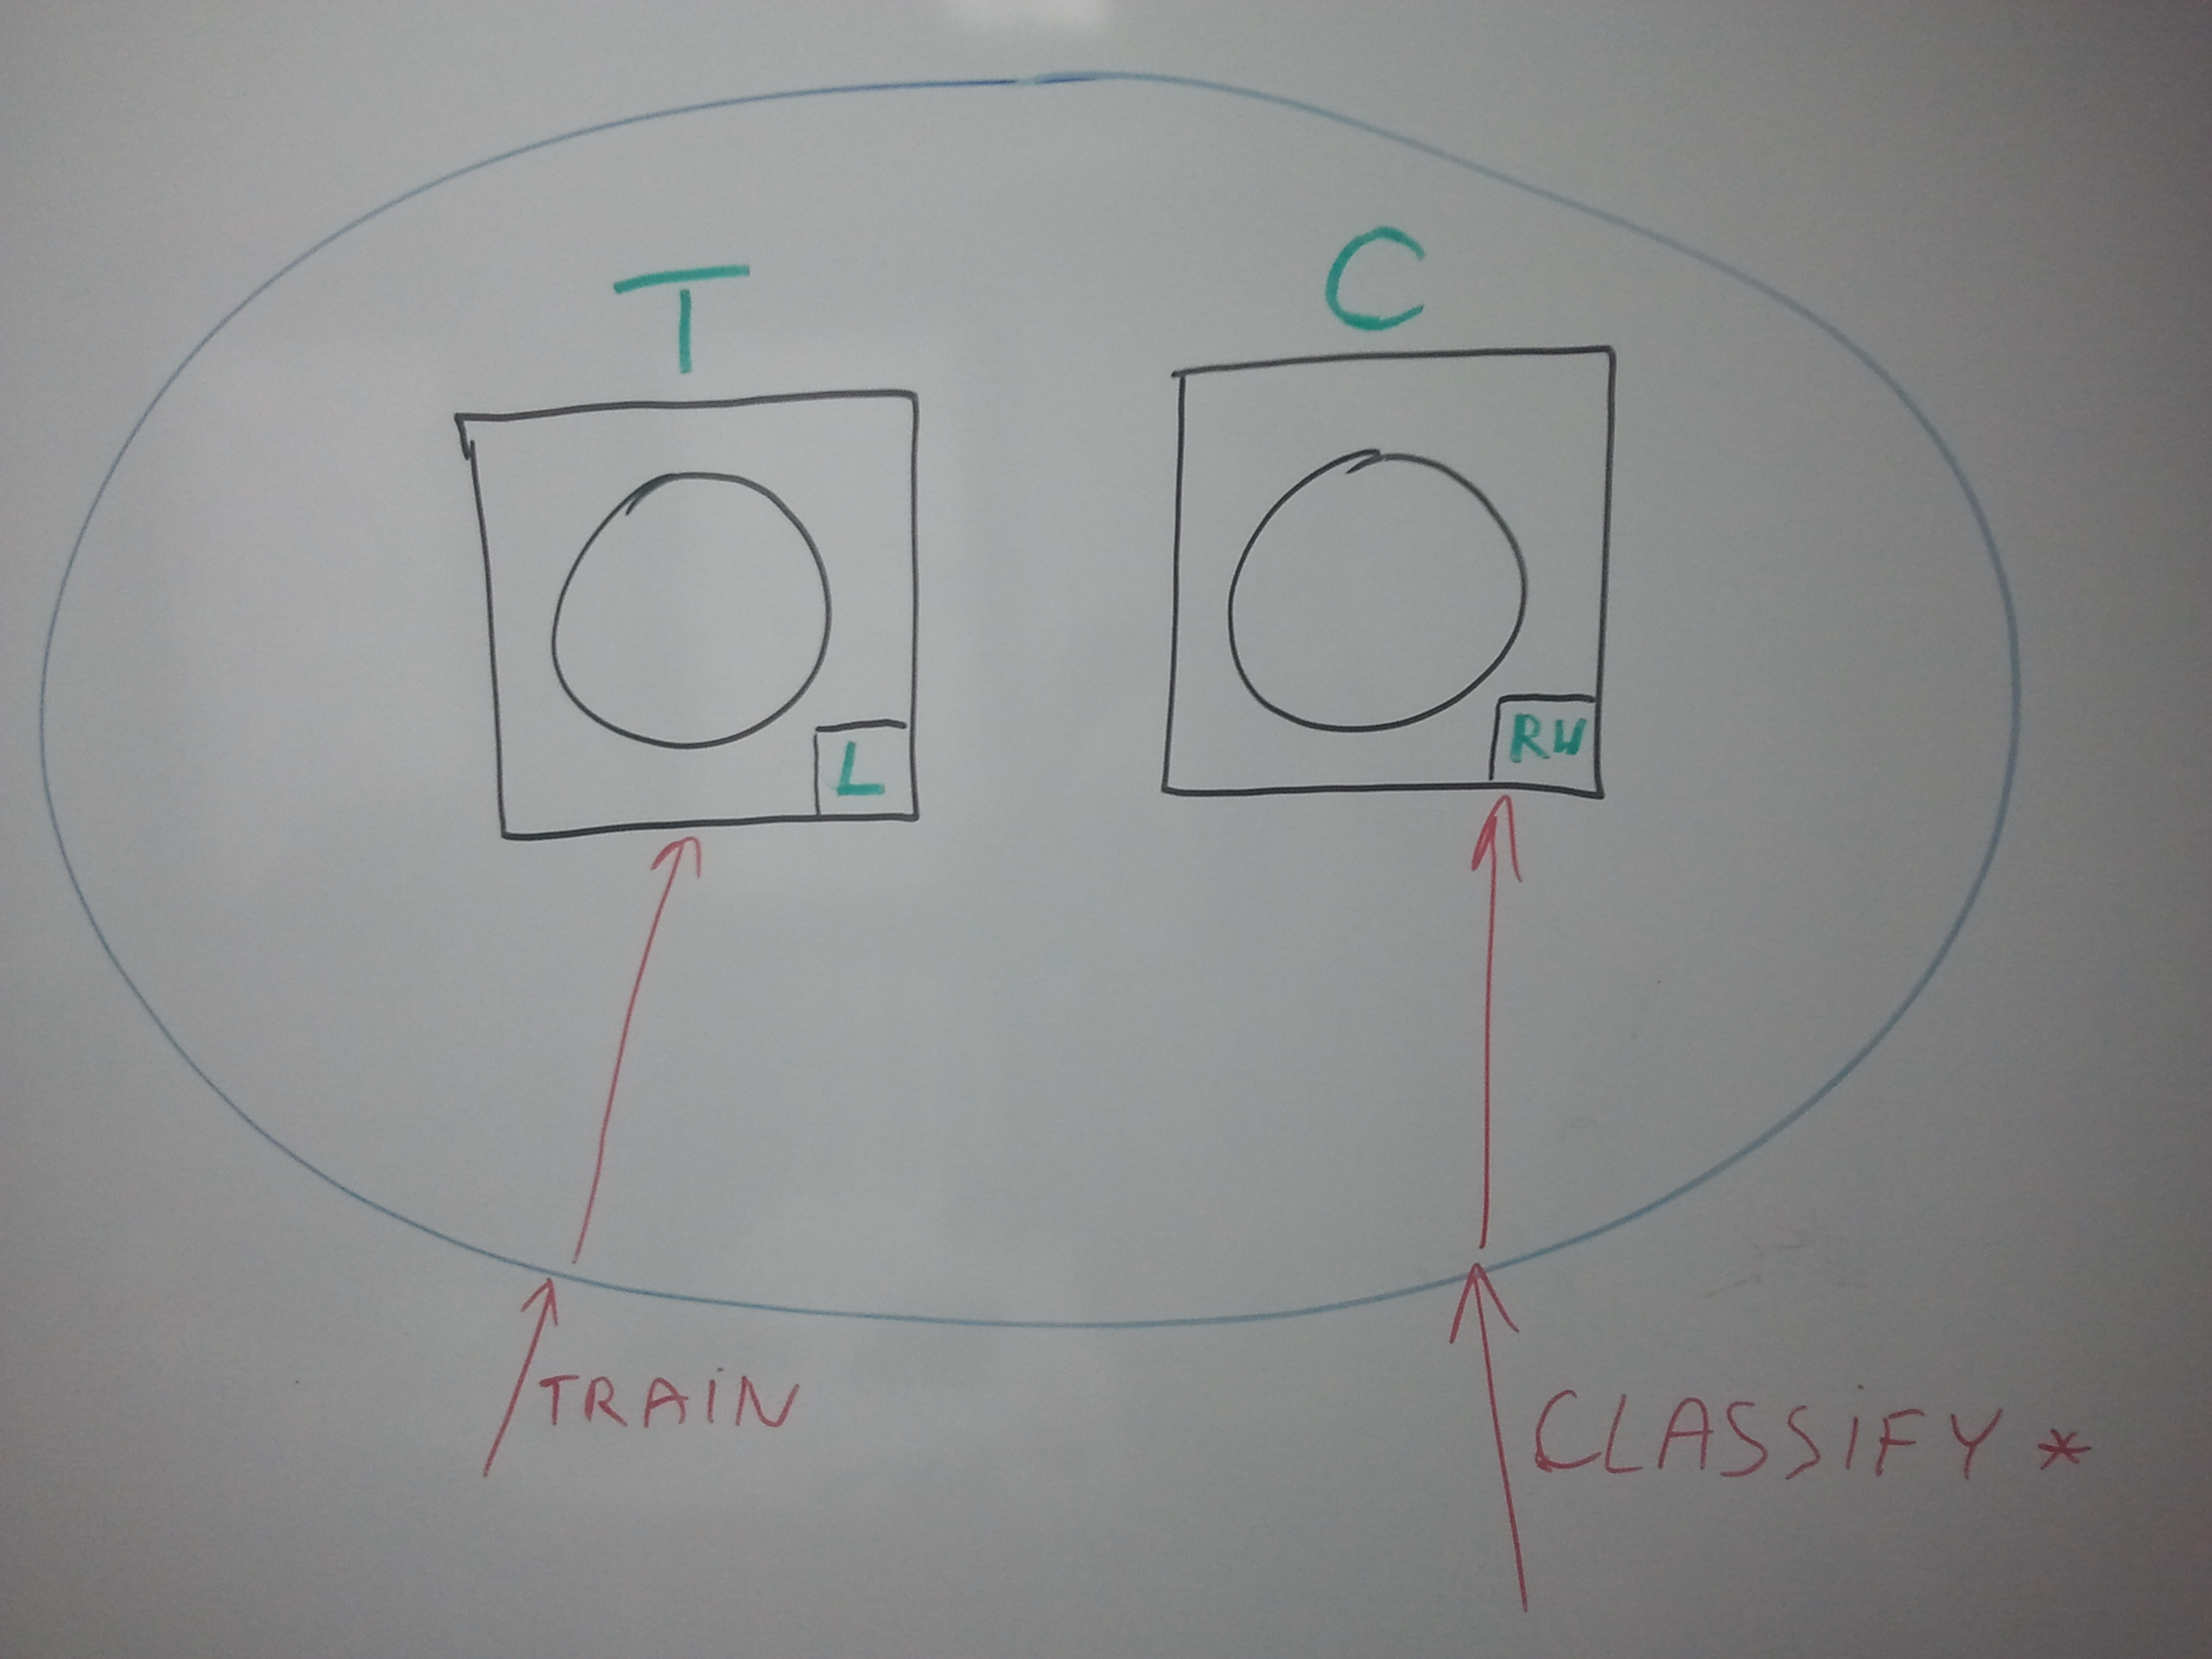
\includegraphics[scale=0.1]{overall.jpg} 
\end{center}
\end{frame}

\begin{frame}
\frametitle{Classify}
\begin{center}
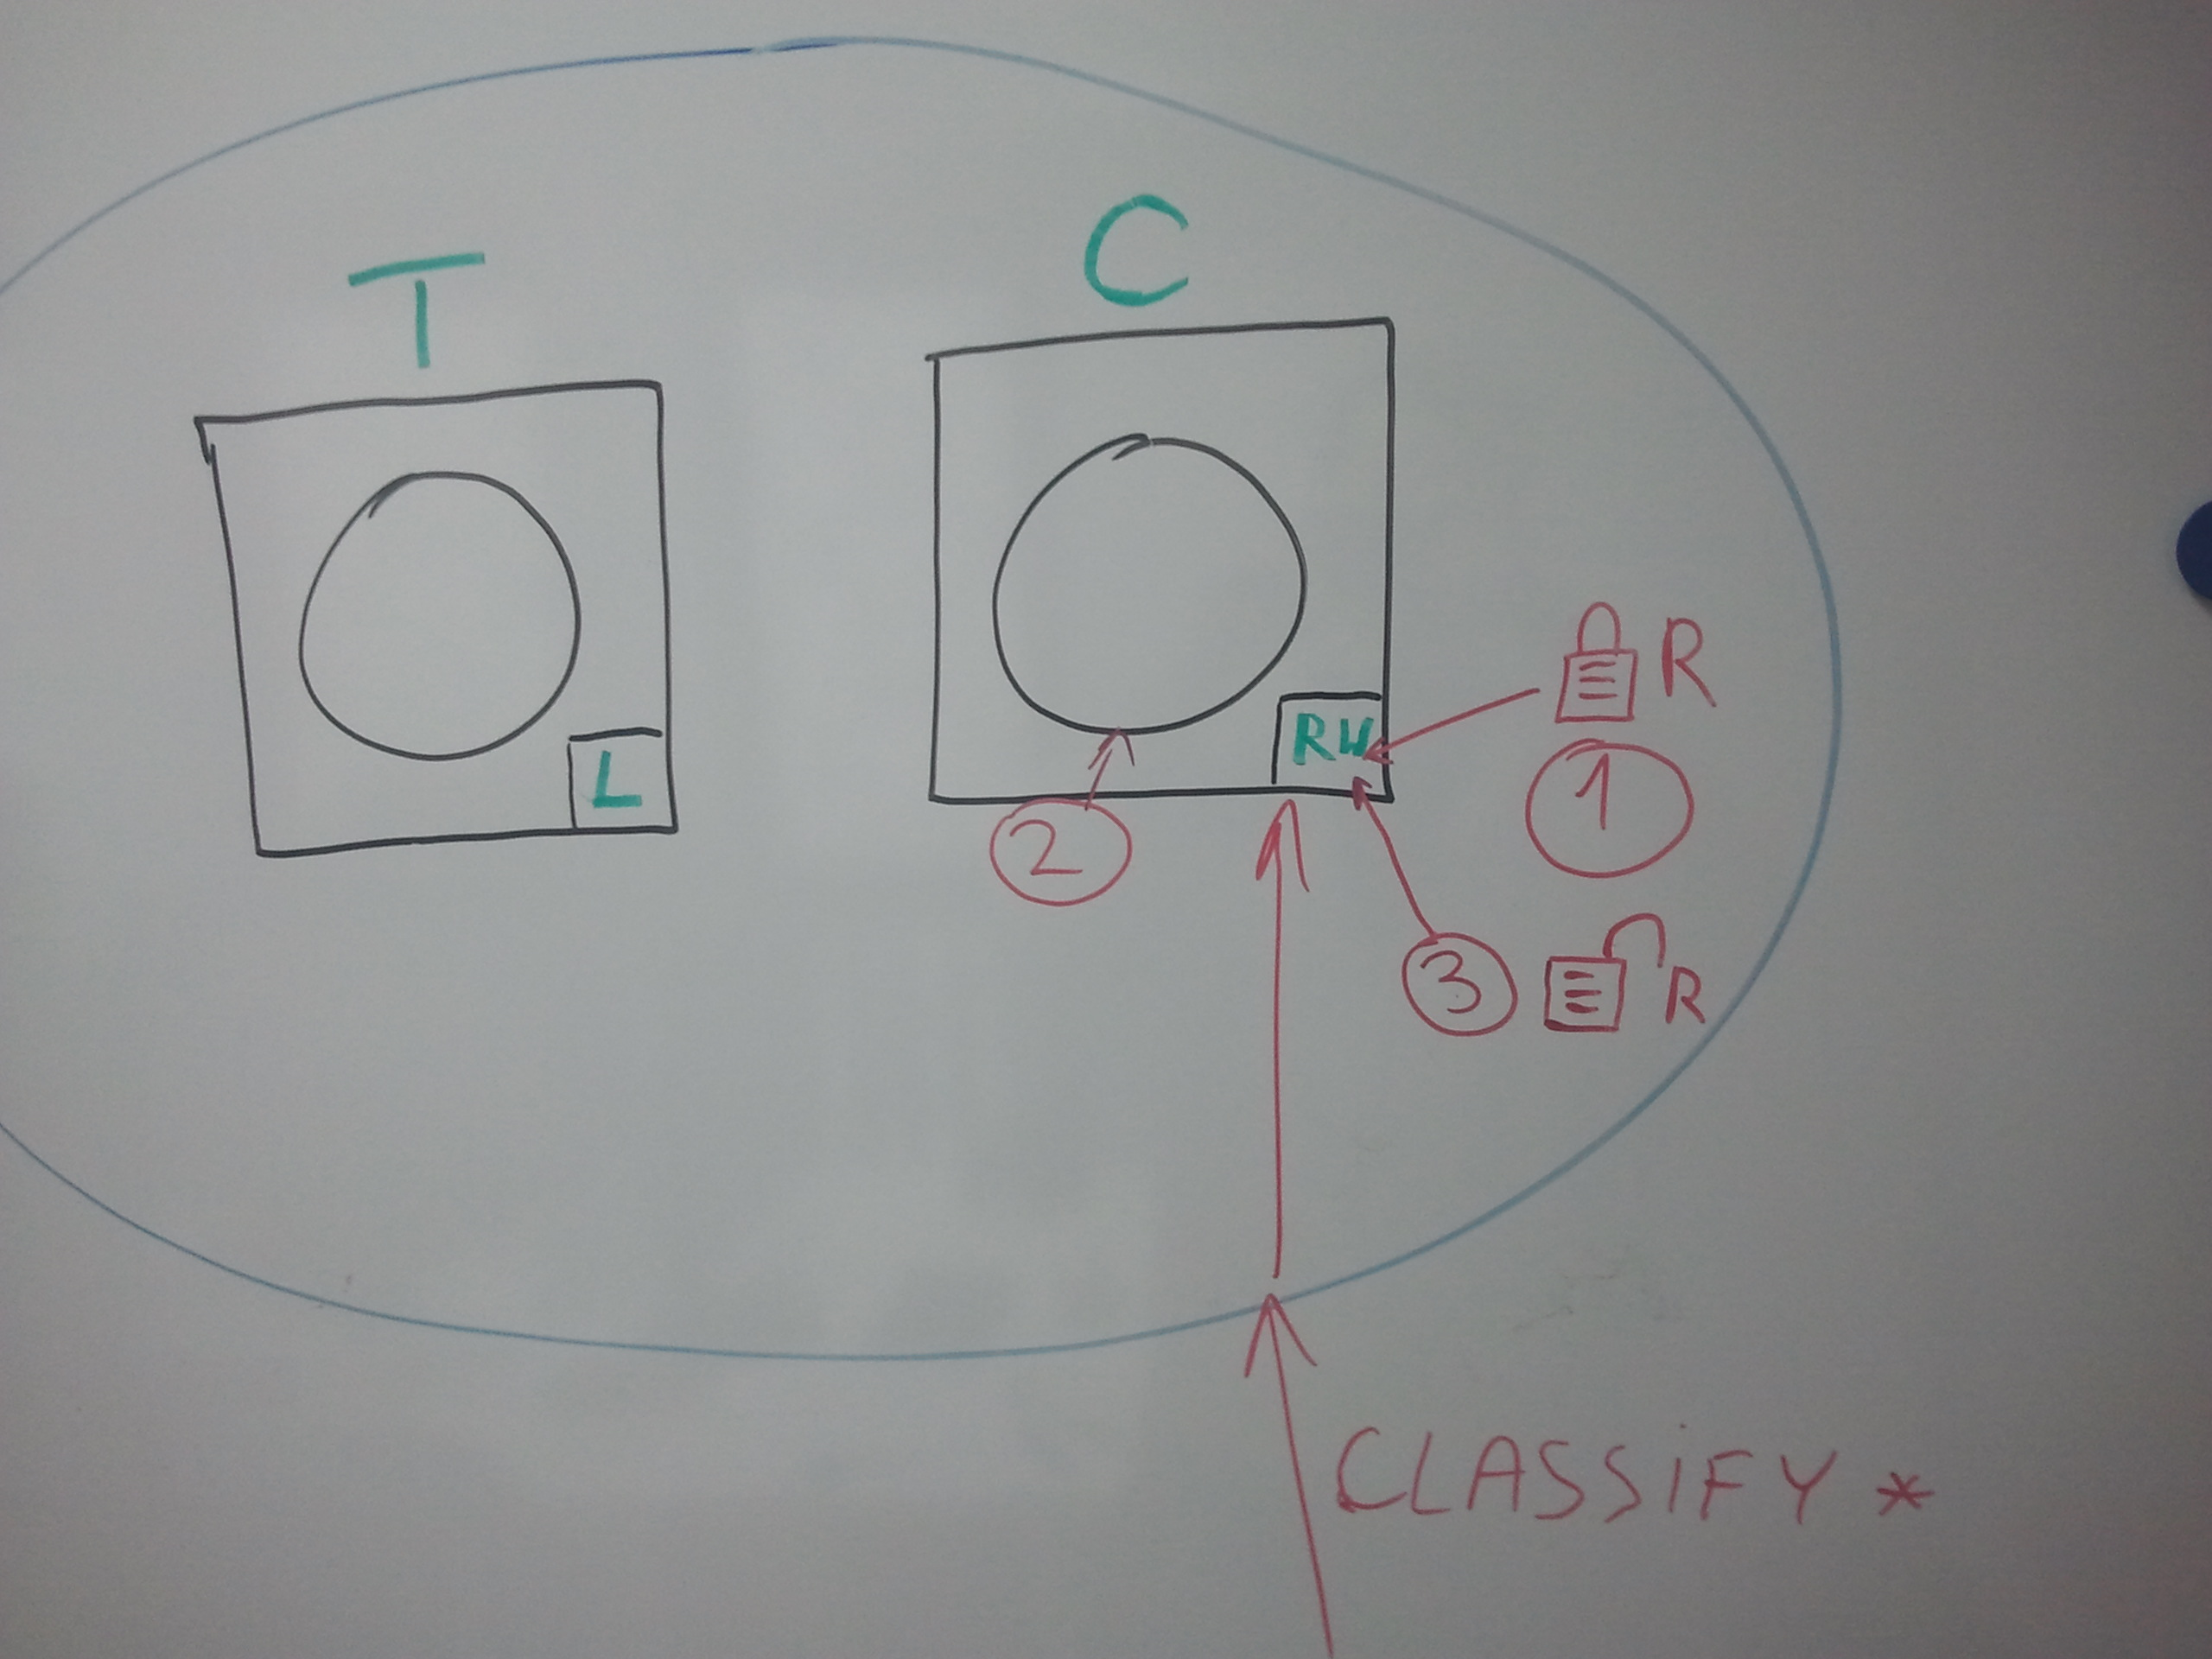
\includegraphics[scale=0.1]{classify.jpg} 
\end{center}
\end{frame}

\begin{frame}
\frametitle{Train}
\begin{center}
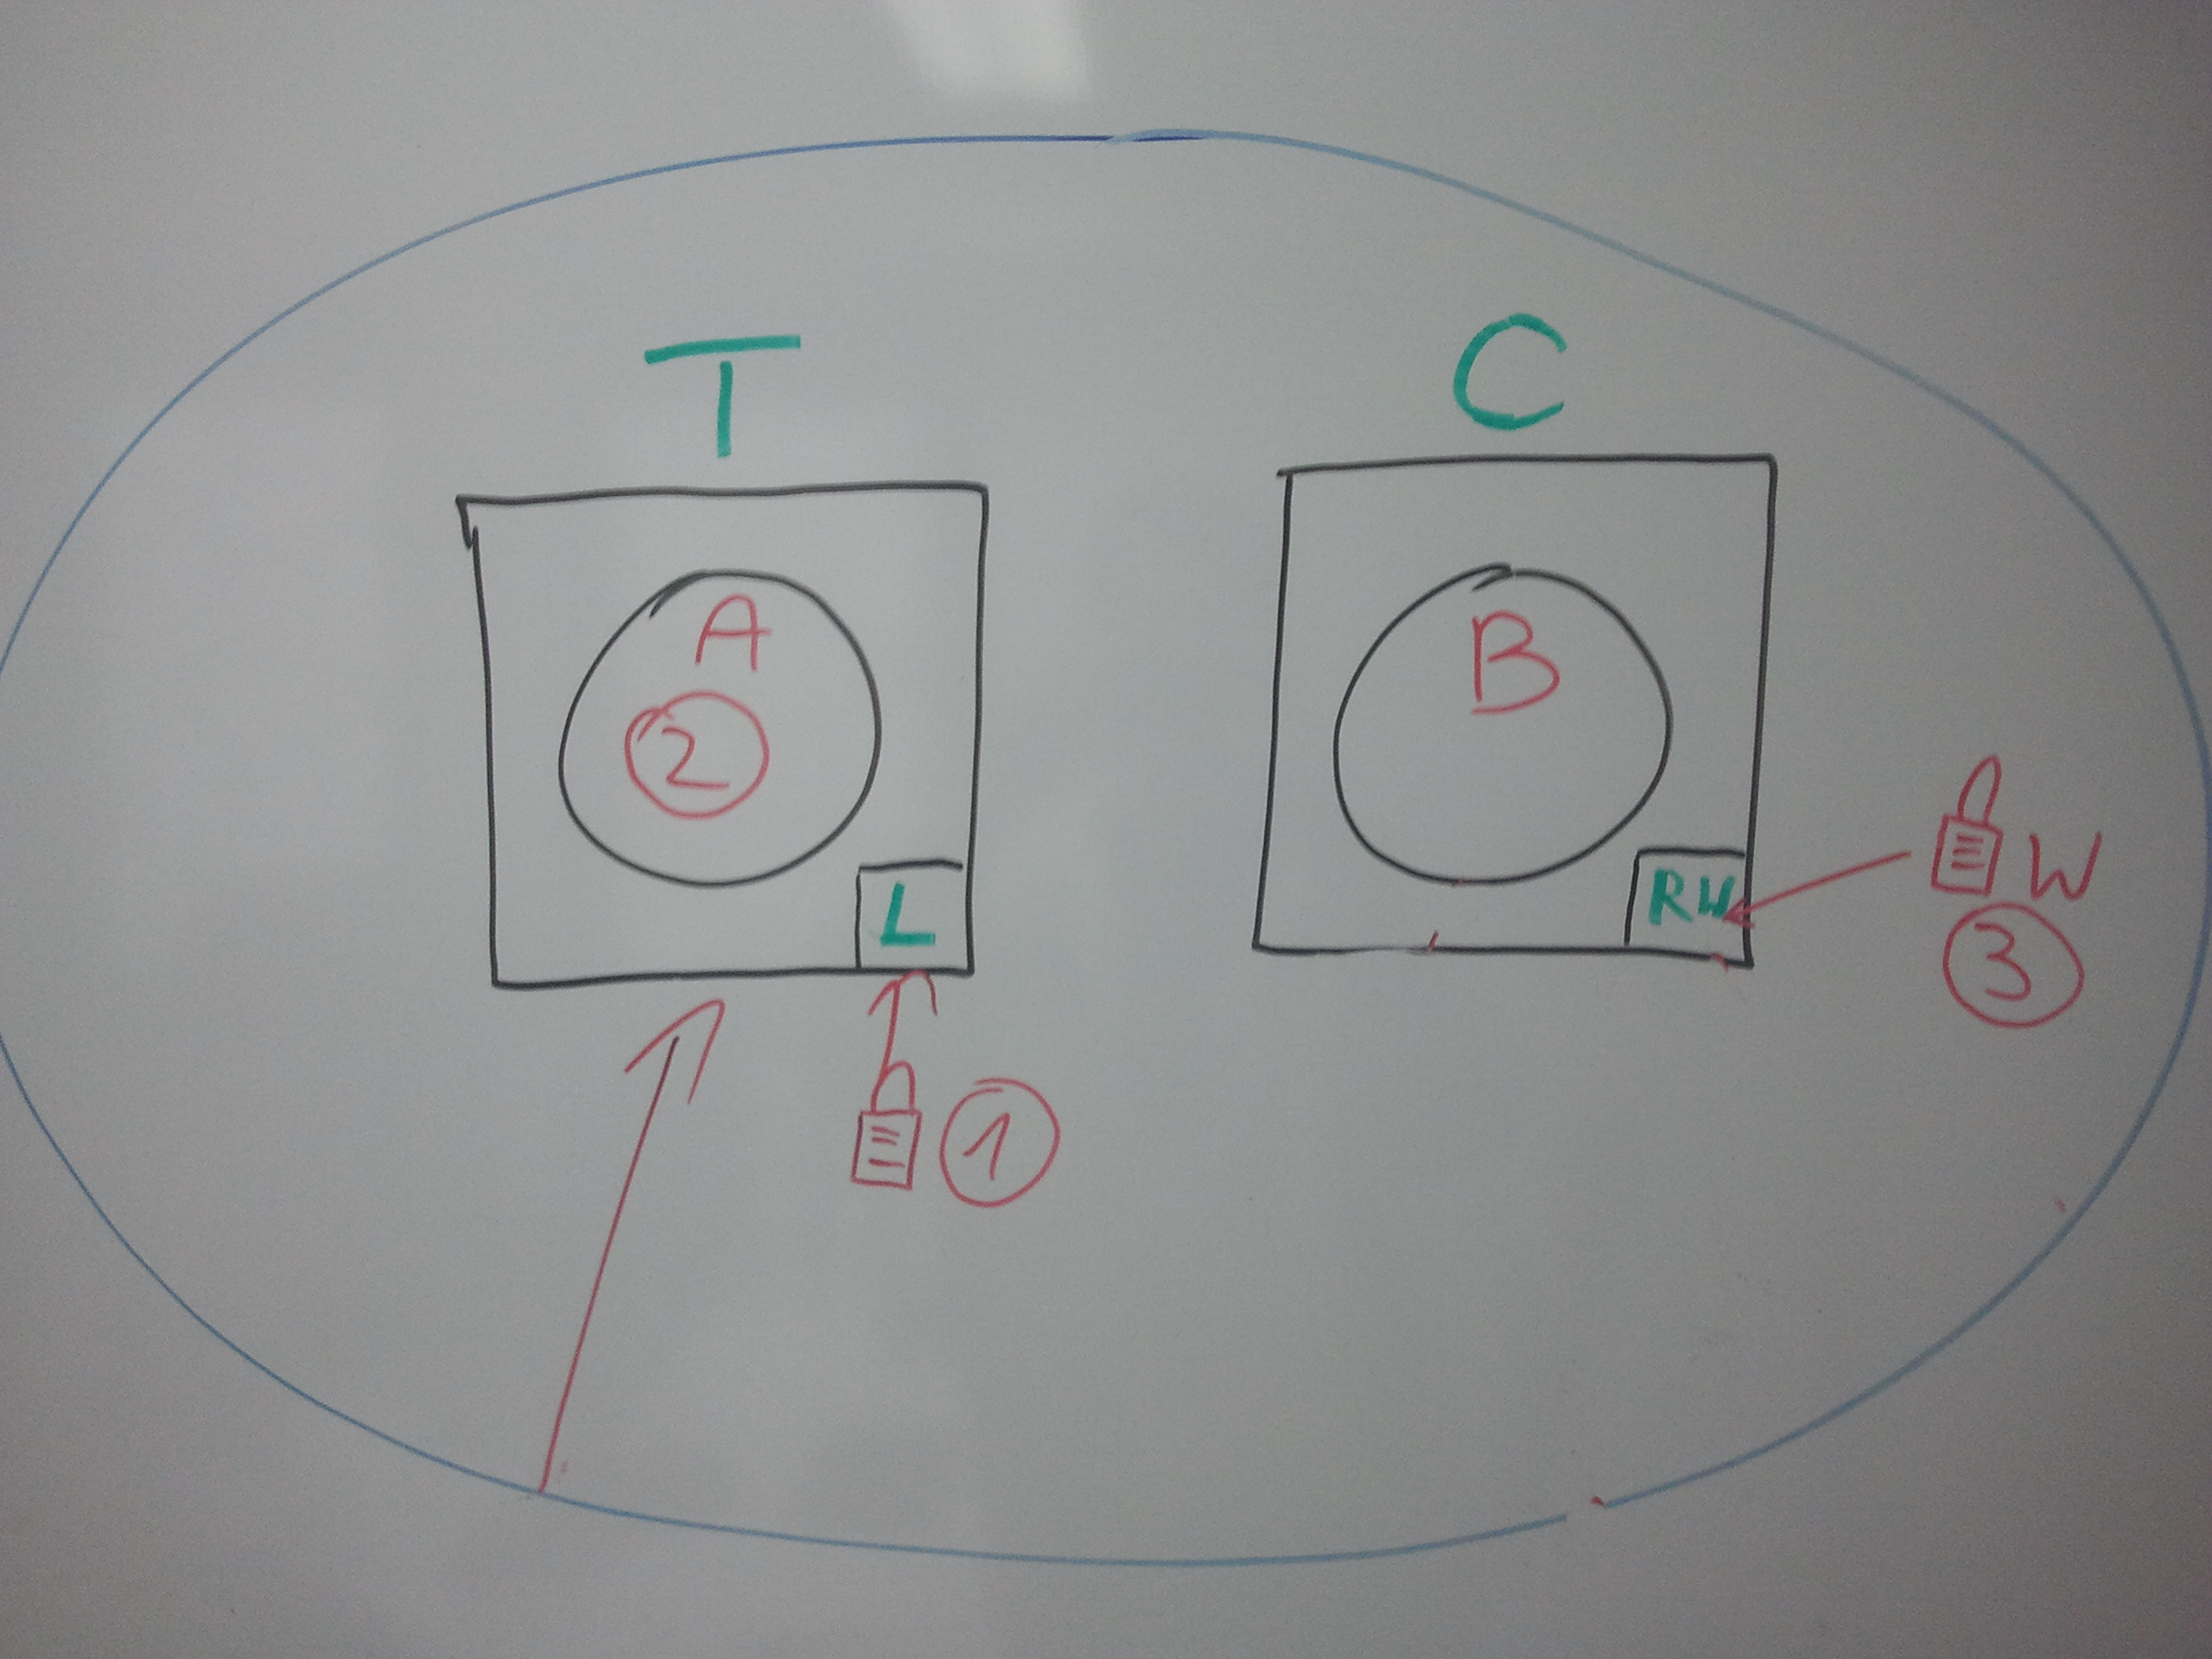
\includegraphics[scale=0.1]{train1.jpg} 
\end{center}
\end{frame}

\begin{frame}
\frametitle{Train}
\begin{center}
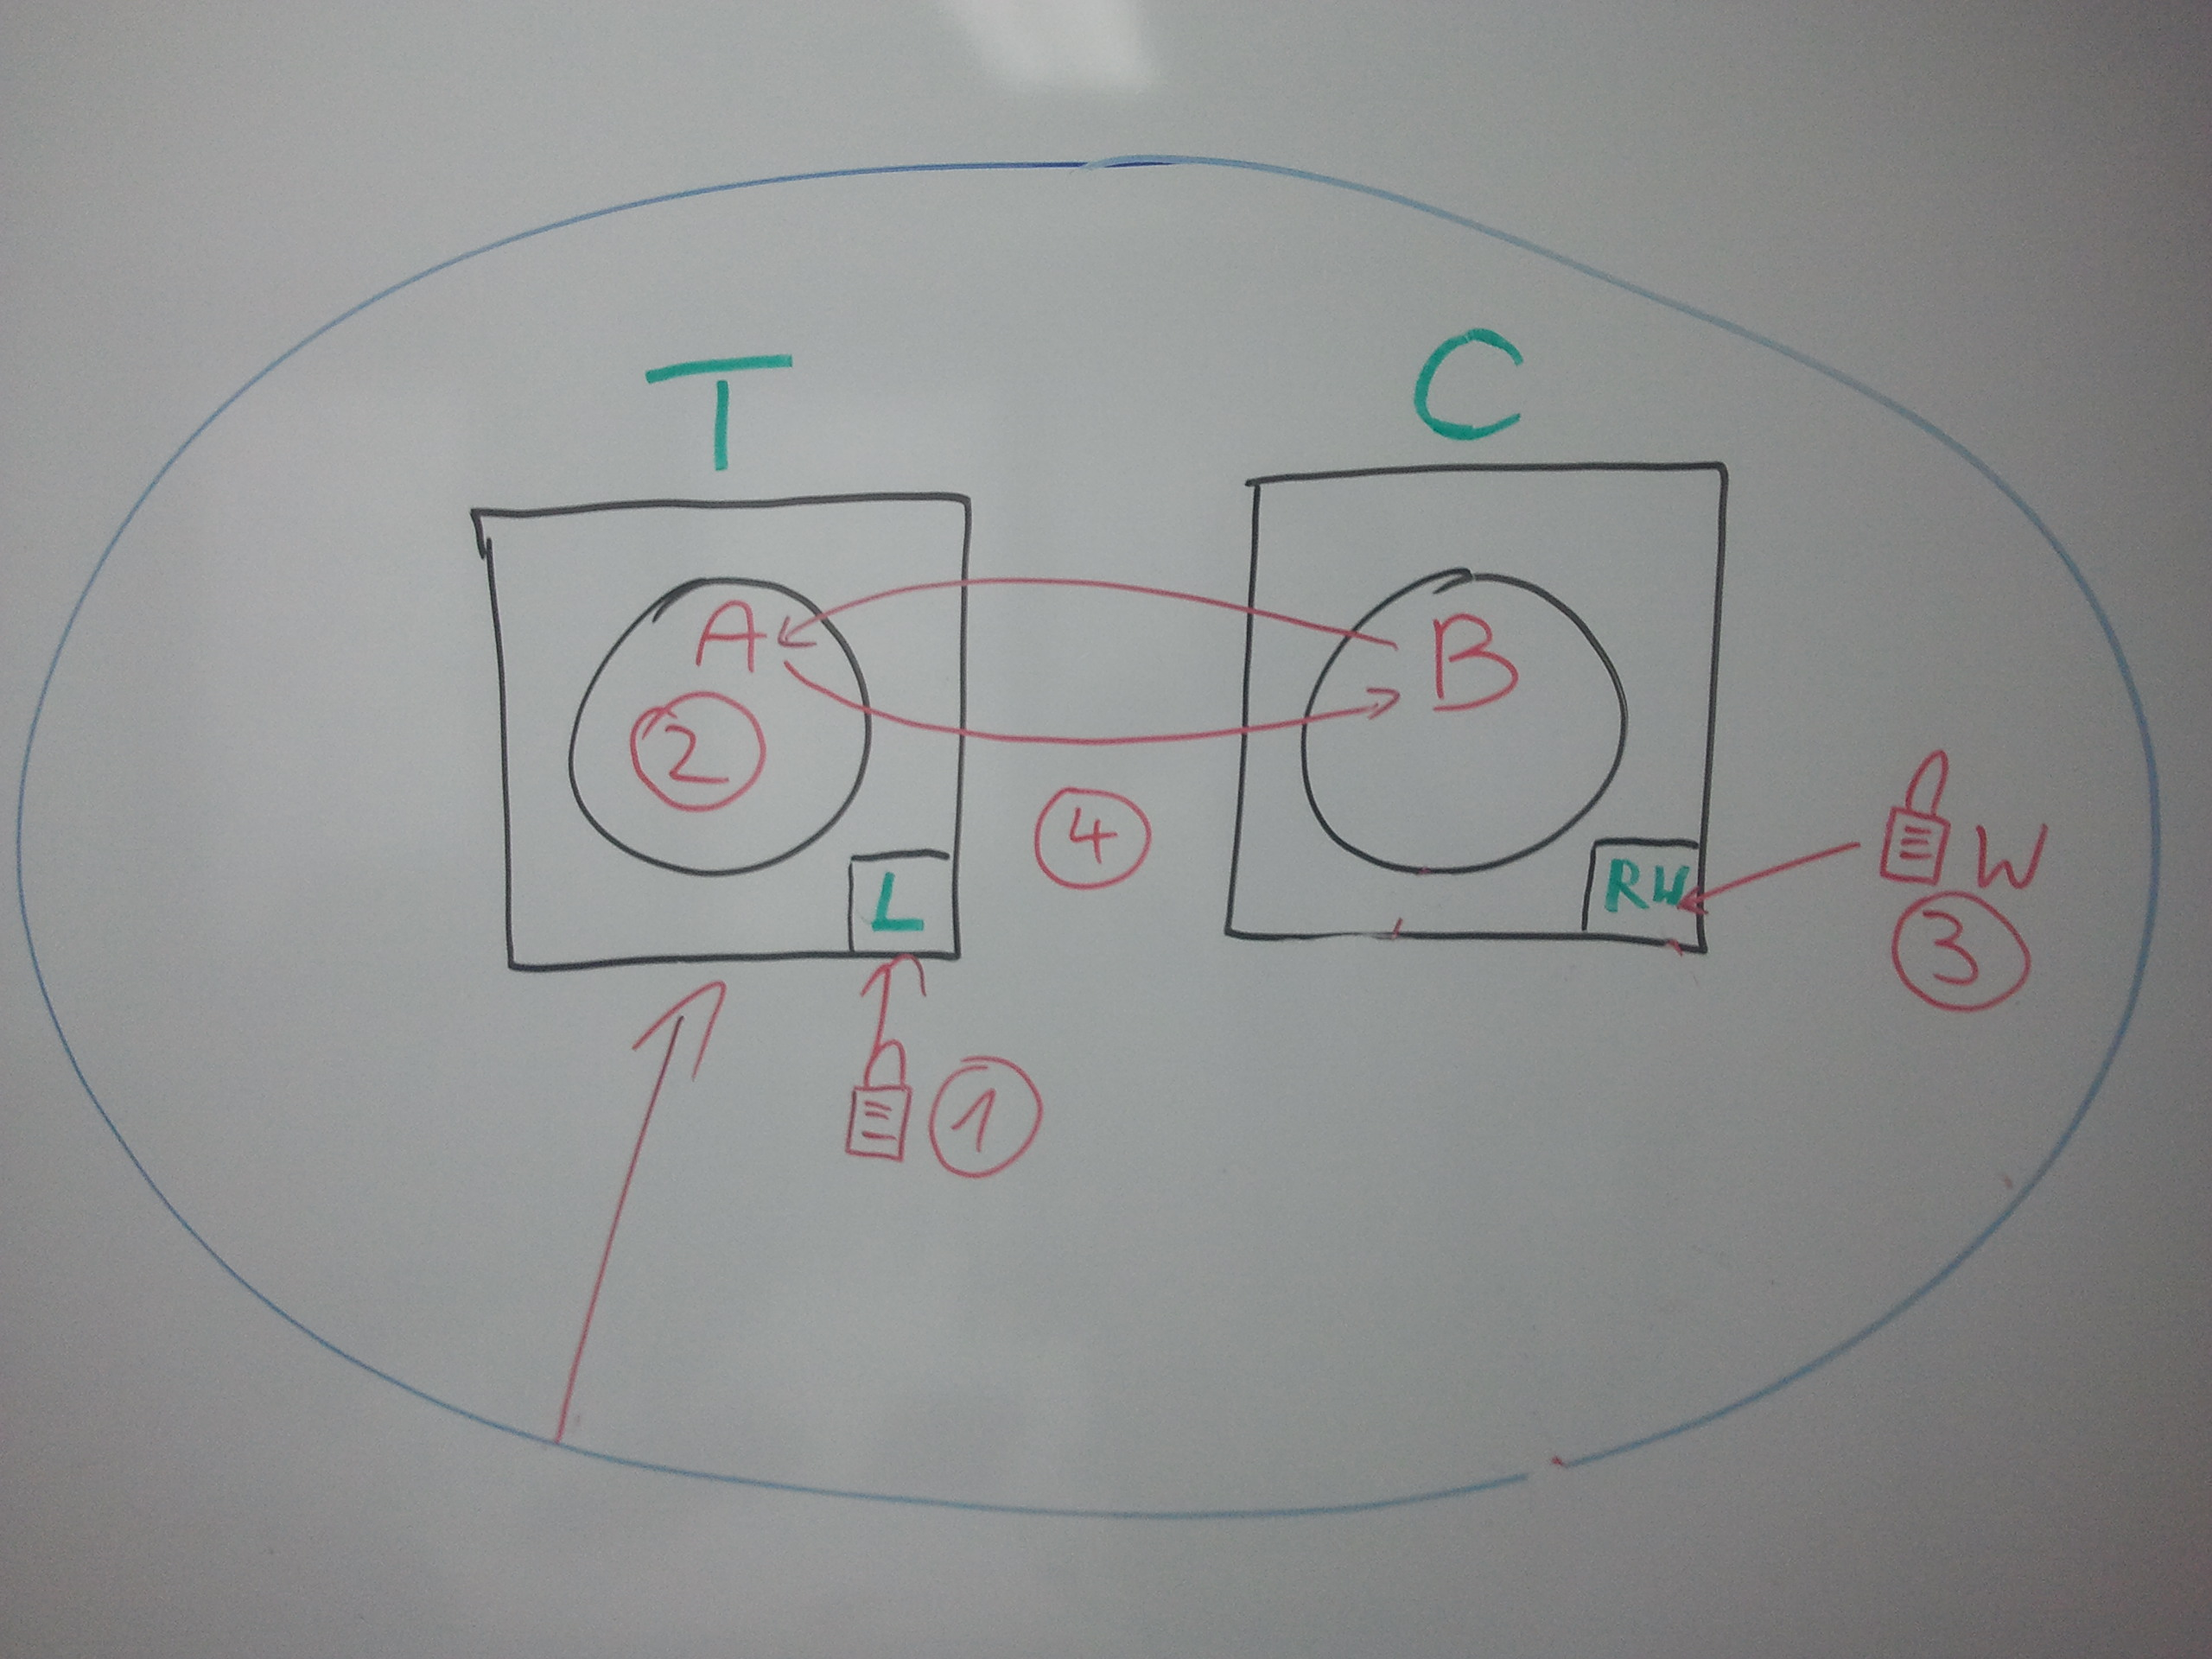
\includegraphics[scale=0.1]{train2.jpg} 
\end{center}
\end{frame}

\begin{frame}
\frametitle{Train}
\begin{center}
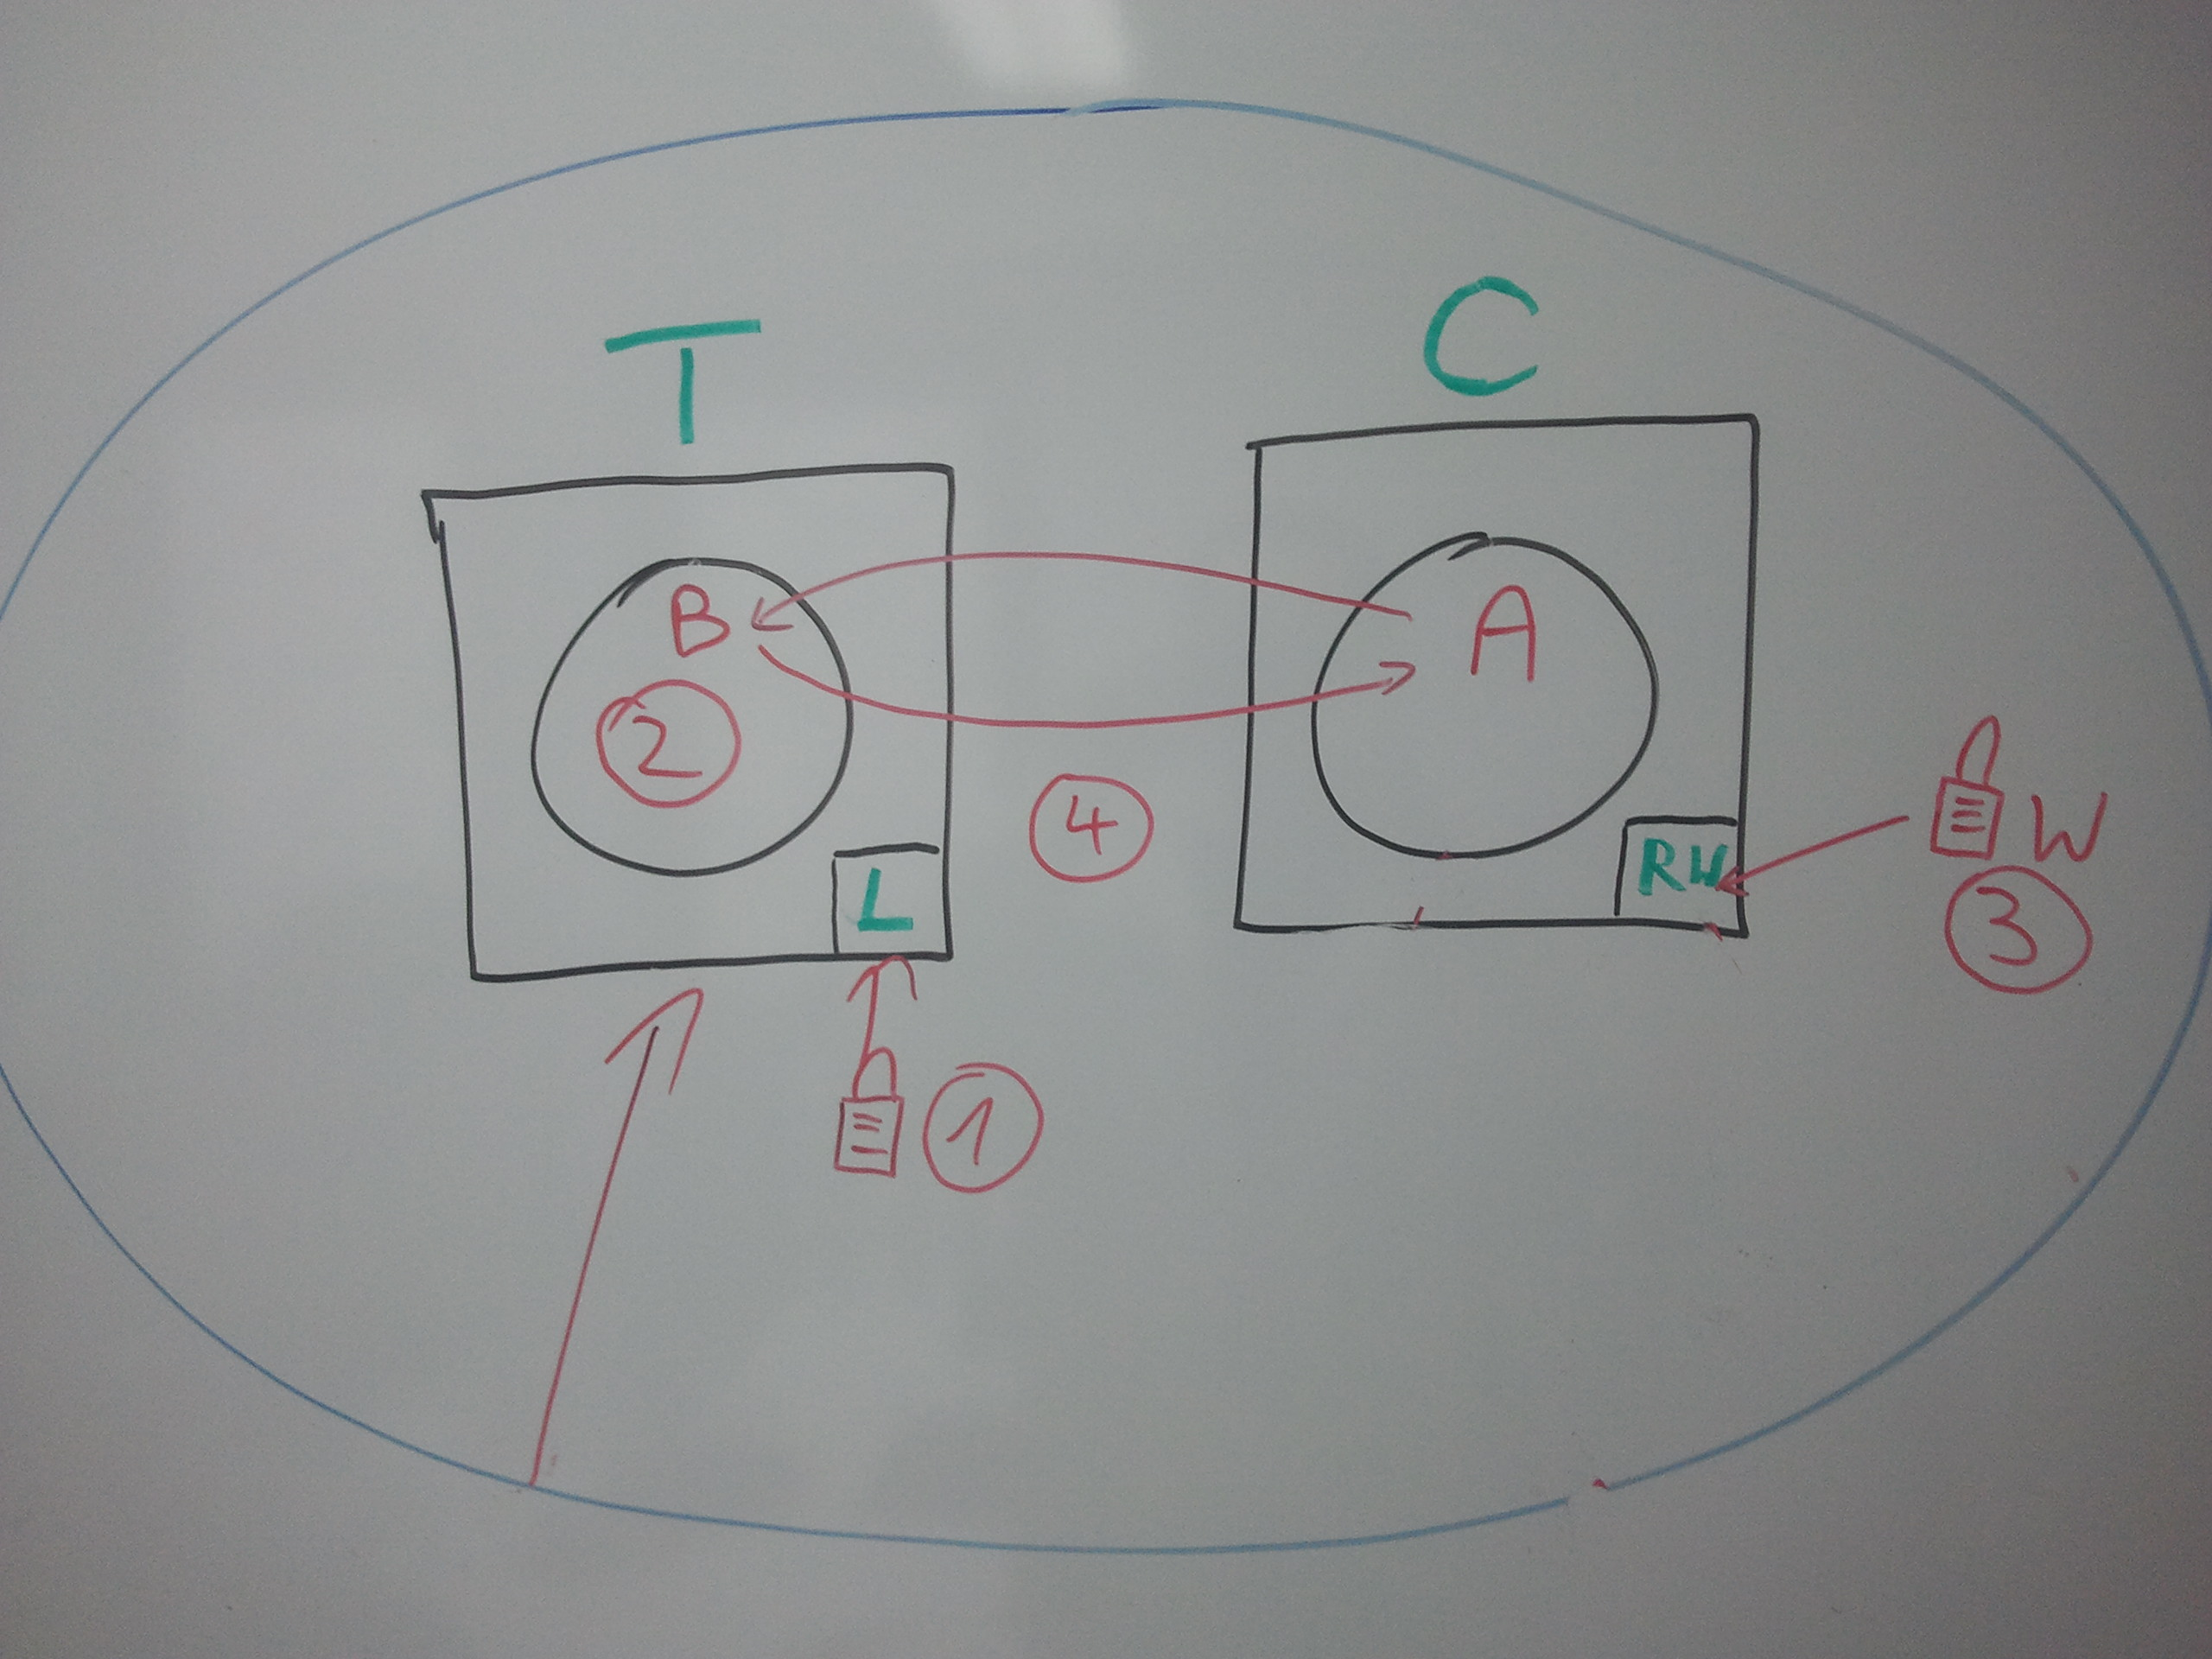
\includegraphics[scale=0.1]{train3.jpg} 
\end{center}
\end{frame}

\begin{frame}
\frametitle{Train}
\begin{center}
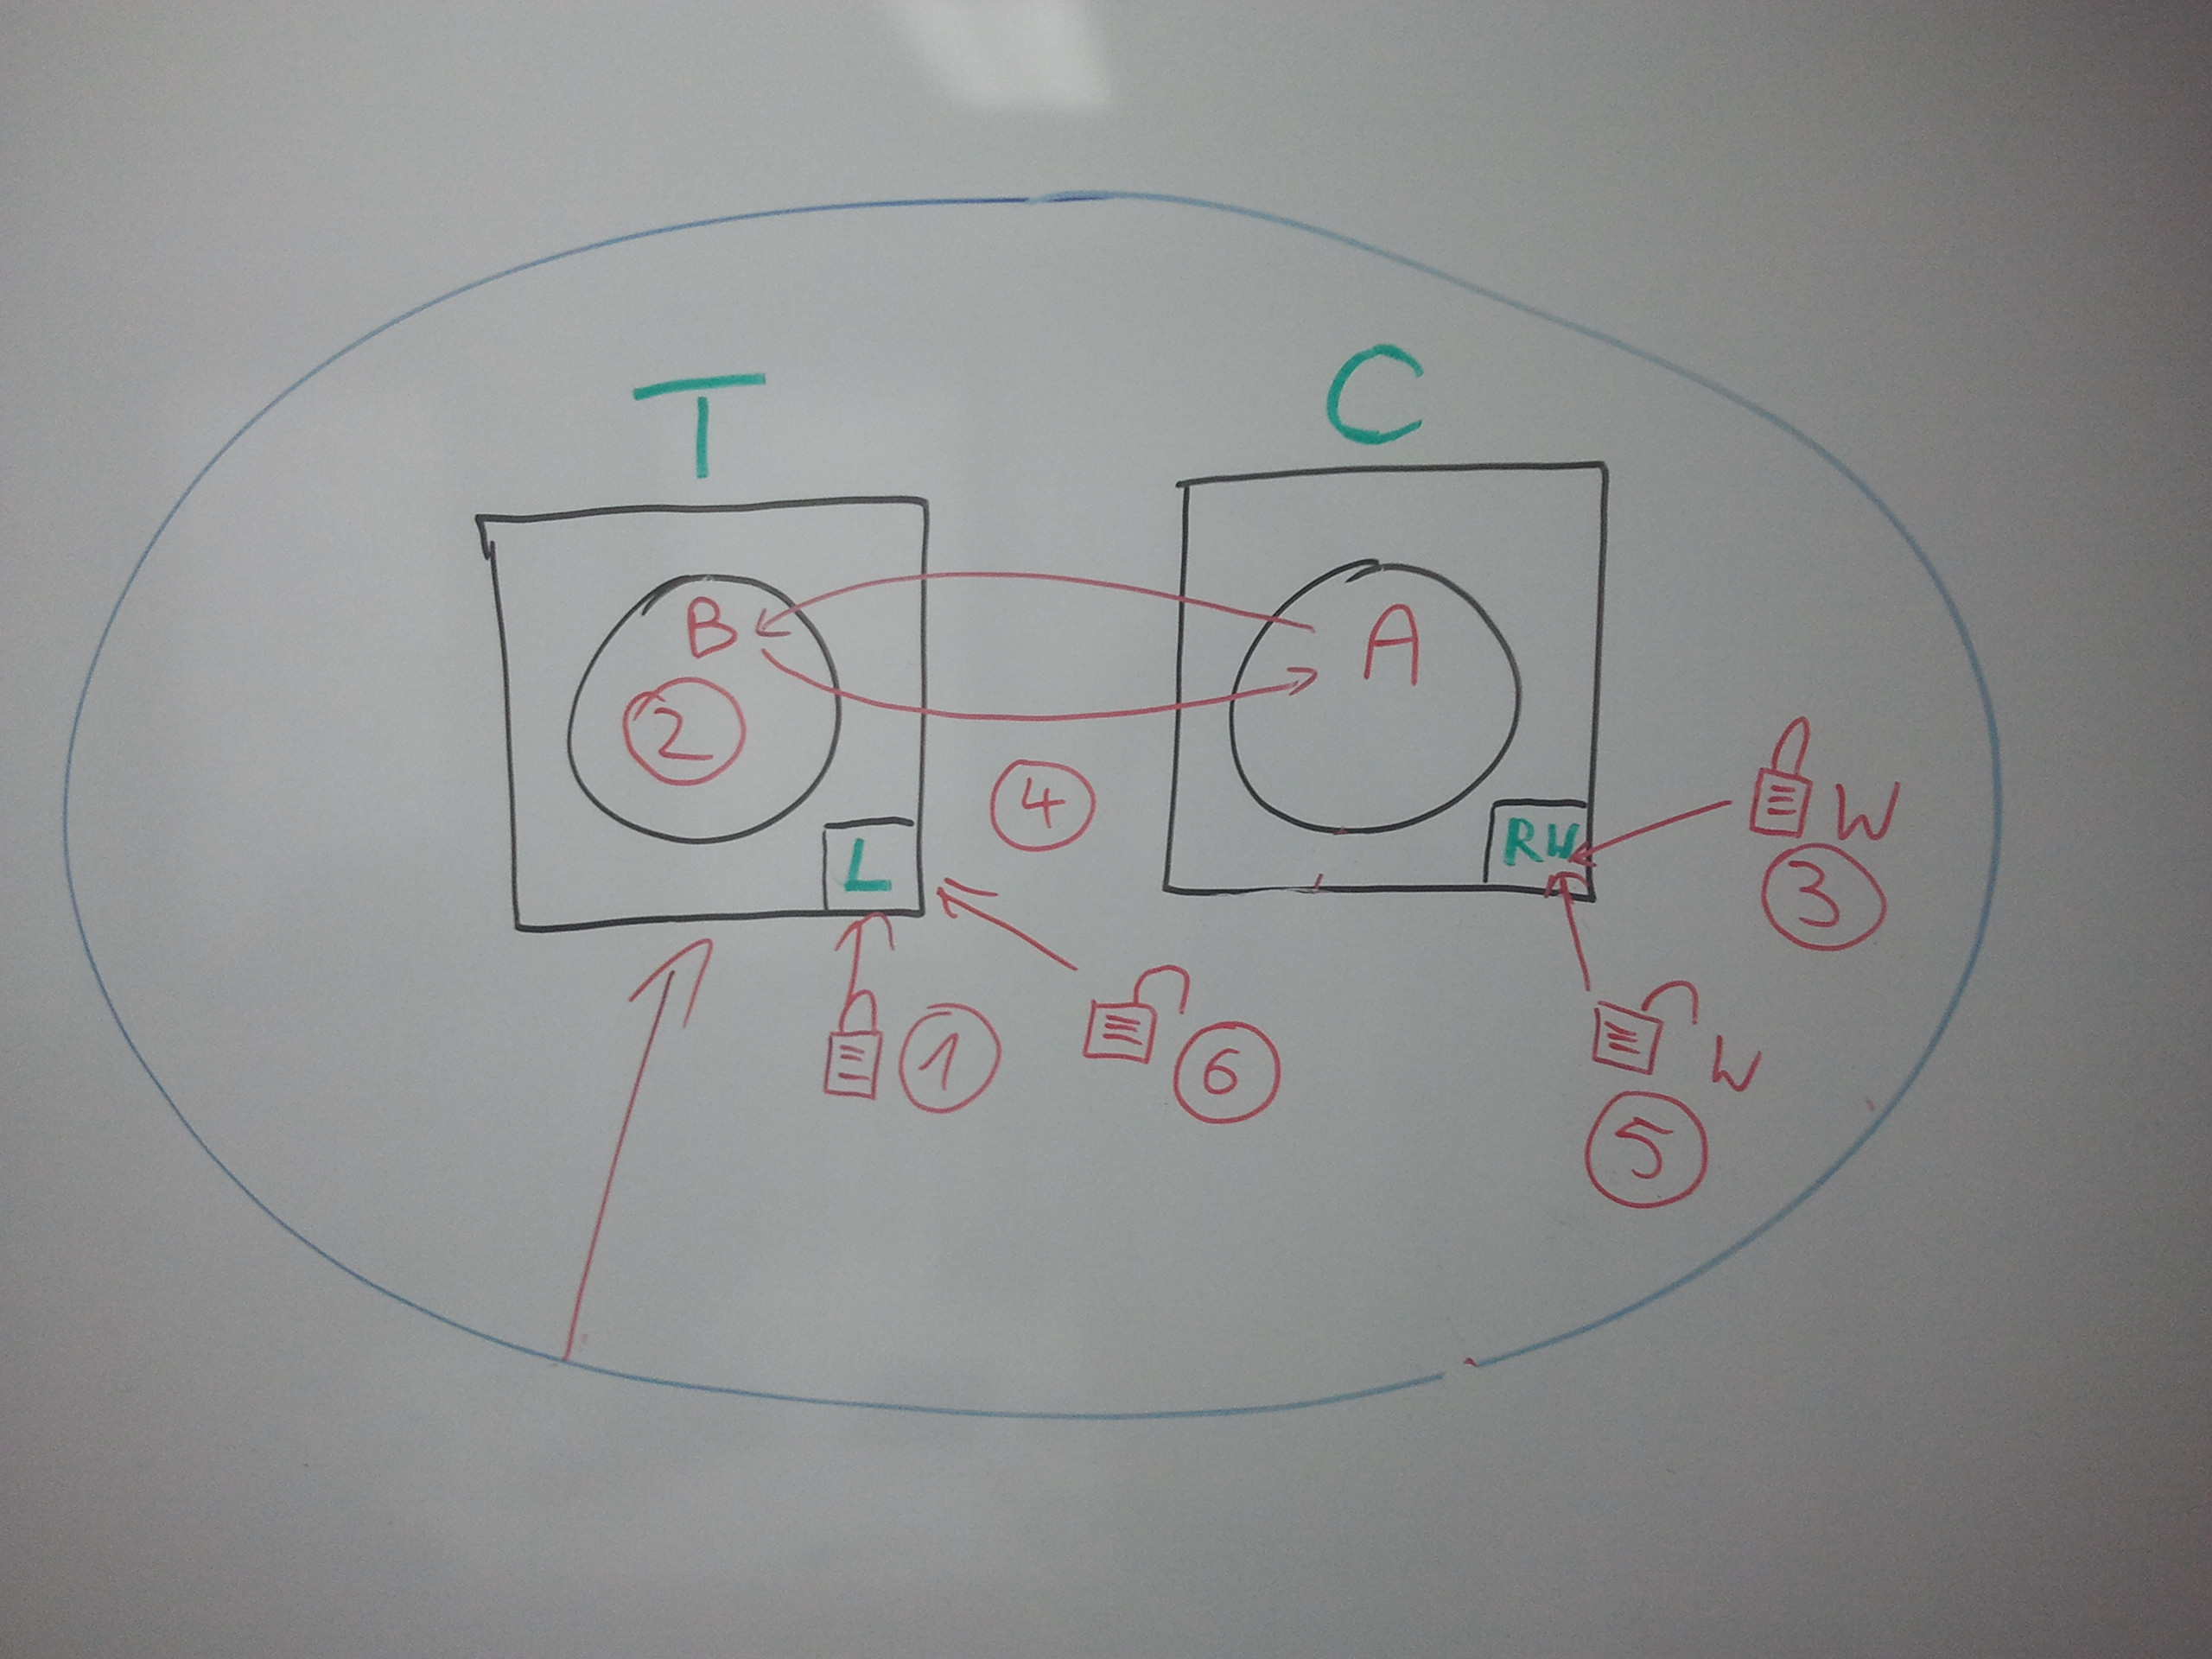
\includegraphics[scale=0.1]{train4.jpg} 
\end{center}
\end{frame}


\begin{frame}
\frametitle{Overall view}
\begin{center}
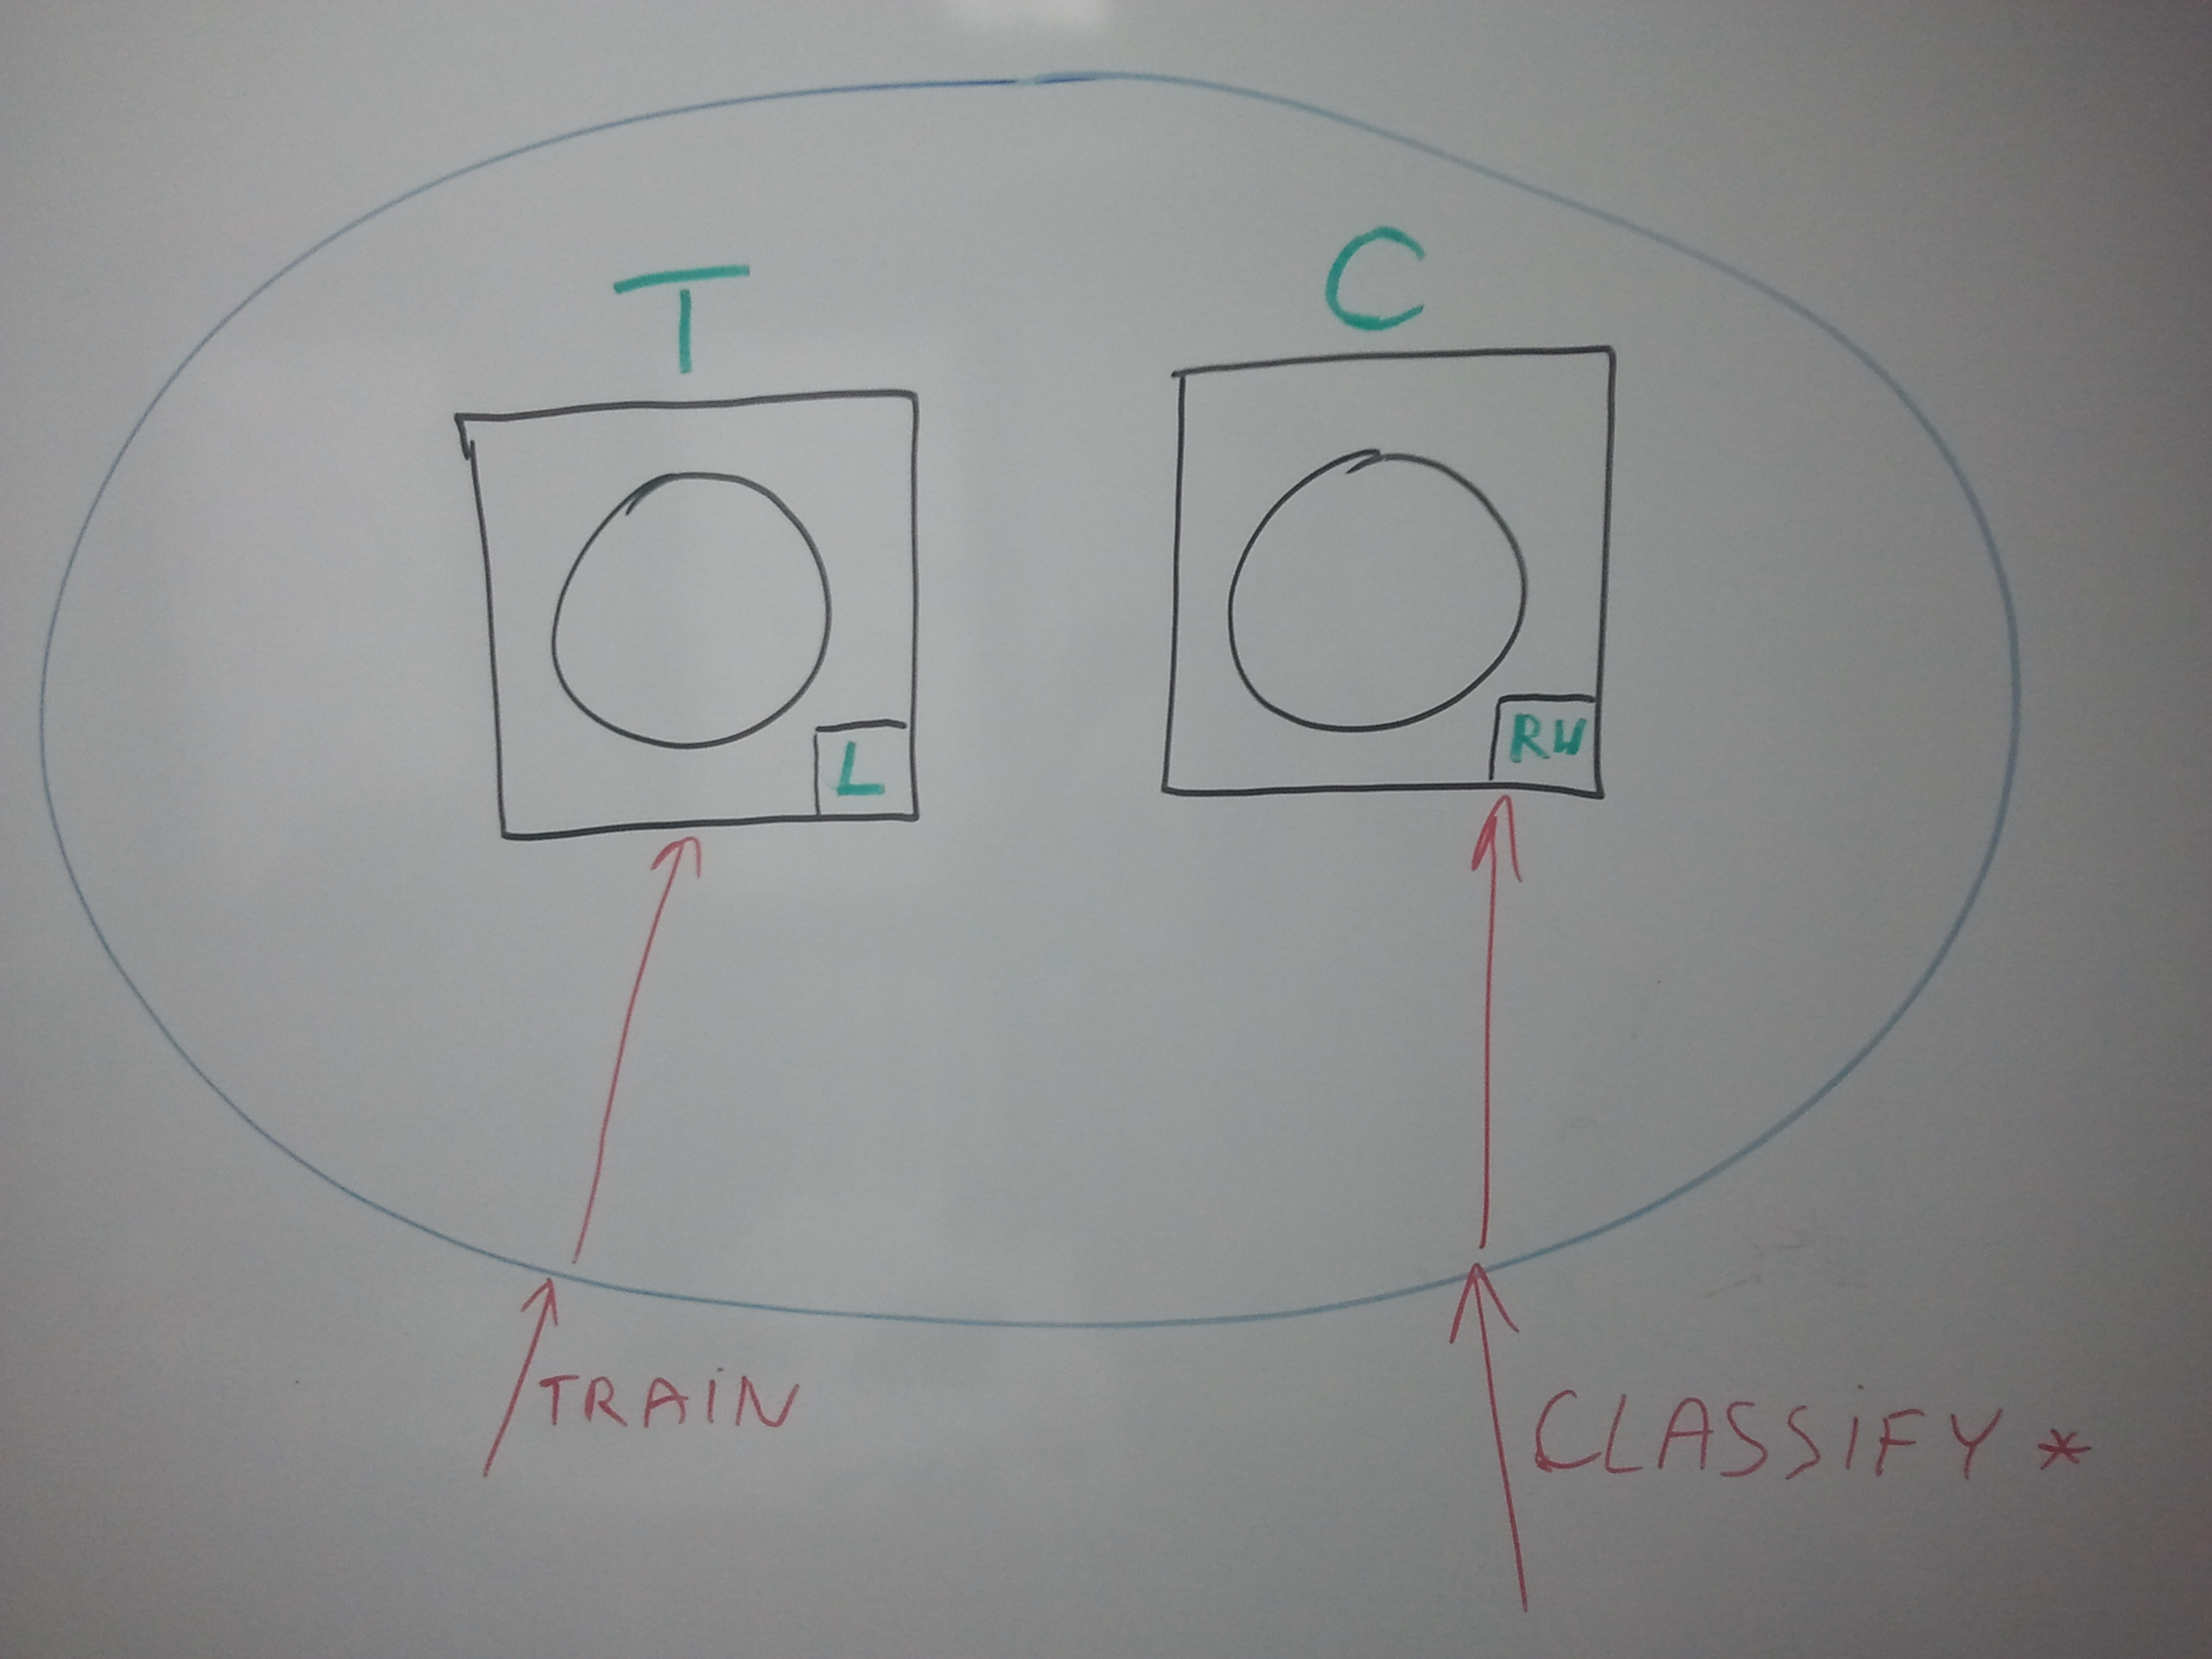
\includegraphics[scale=0.1]{overall.jpg} 
\end{center}
\end{frame}


\begin{frame}
\begin{block}{Summary}
\begin{itemize}
 \item $+$ no long reads
 \item $+$ no need to know how to construct classifier - they are given at initialization
 \item $-$ doubles memory/resource requirements
\end{itemize}
\end{block}
\end{frame}
\section{Some notes}

\begin{frame}
\begin{itemize}
 \item 24/7 matches \emph{decorator patter} schema
 \item Python stdlib lacks synchronization of not related processes
 \item Java stdlib implements RW synchronization only with locks
\end{itemize}
\end{frame}

\begin{frame}
\begin{center}
\Huge{Q \& m A}

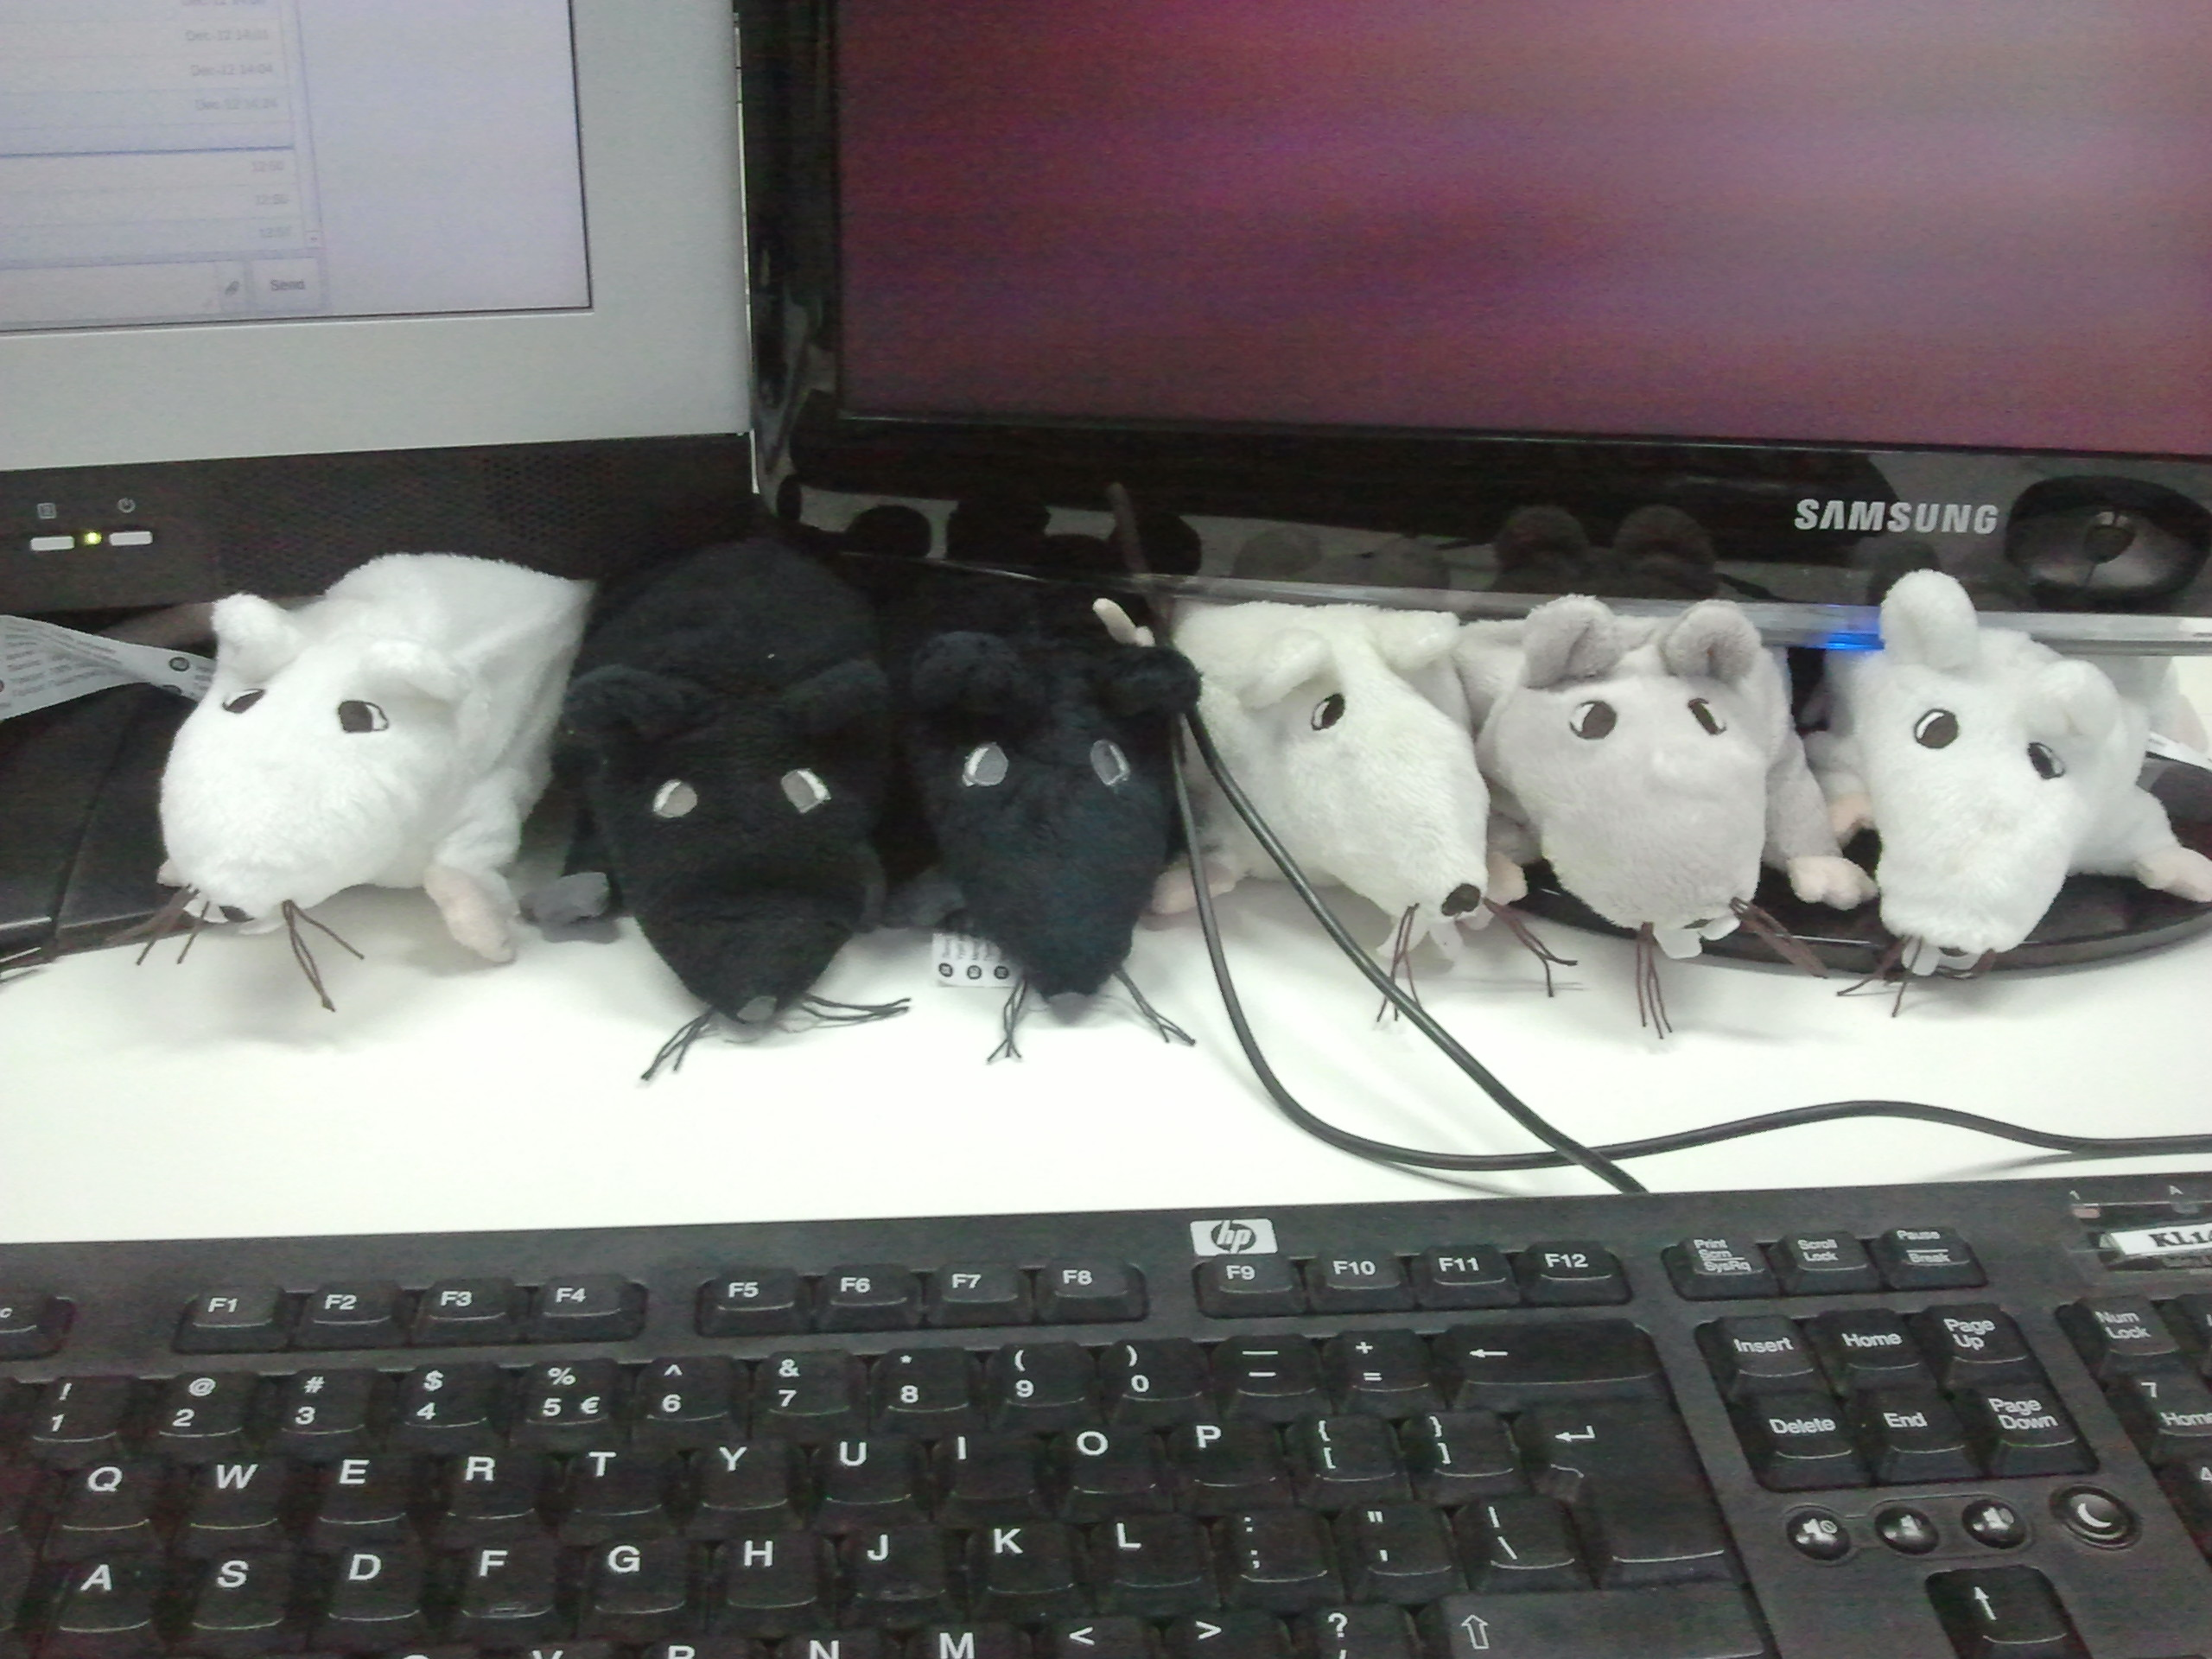
\includegraphics[scale=0.1]{questions.jpg} 

\end{center}

\end{frame}

\begin{frame}

Next time: slooooow readers ...

\begin{center}
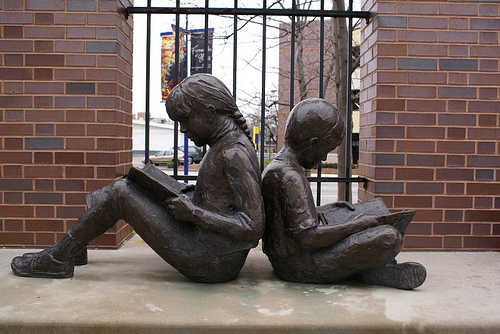
\includegraphics[scale=0.5]{slow_readers.jpg} 

\end{center}
\end{frame}
\end{document}
